L'énergie nucléaire présente l'avantage de nécessiter considérablement moins de métaux critiques que l'éolien et le photovoltaïque. Cependant trois points sont à surveiller pour évaluer le risque géopolitique du nucléaire : l'approvisionnement en uranium, la production du combustible et la construction des réacteurs.\smallbreak
L'extraction d'uranium ne présente actuellement pas de risque géopolitique majeur. Les réserves actuelles donnent de la visibilité sur la satisfaction de la demande sur plusieurs dizaines d'années. La prodution d'uranium se répartit sur quatre continents (figure \ref{fig:uranium}).\smallbreak
Le prix de l'uranium sur le marché spot peut connaître des épisodes de volatilité. Mais d'une part, l'uranium représente un coût faible dans le coût de production d'énergie nucléaire, d'autre part, une portion significative des échanges d'uranium se font sur des marchés de long terme. Par ailleurs, des gisements secondaires d'uranium sont disponibles grâce à l'uranium appauvri, au retraitement de combustible usé et le démantèlement d'armes nucléaire.\smallbreak

La fabrication du combustible se compose de trois étapes clés - conversion, enrichissement, transformation - dont le nombre d'acteurs est limité (figure \ref{fig:combustible}).\smallbreak
L'étape de conversion permet de transformer l'uranium de sortie site minier (yellow cake) en hexafluorure d’uranium (UF6). Cette transformation est nécessaire pour permettre l'étape d'enrichissement. L'enrichissement sert à augmenter la concentration en Uranium 235 de 0.7\% à environ 4\%. La transformation convertit l'hexafluore d'uranium en dioxyde d'uranium (UF2), l'uranium obtenu est compressé en pastilles. Certaines technologies nucléaires marginales sur le plan énergétique peuvent avoir un procédé de fabrication du combustible différent. Les pays producteurs de combustible se situent dans des blocs géopolitiques indépendants, ce qui réduit le risque sur l'approvisionnement (\cite{meyer_les_2021}). Cependant le passage d'un fabricant à un autre peut prendre un certain temps mais ce passage est en général techniquement possible à l'image de la Finlande qui fait appel à Westinghouse pour la substitution du combustible Rosatom (\cite{westinghouse_electric_company_helping_2022}).\smallbreak

\begin{figure}[!b]
    \centering
    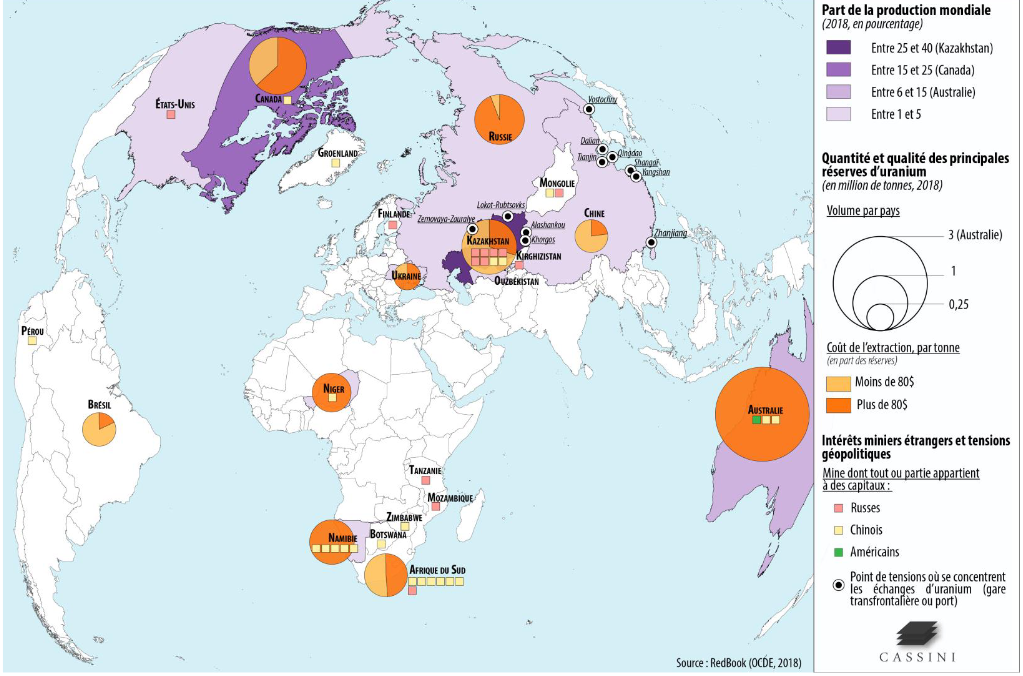
\includegraphics[width=0.95\textwidth]{Images/nucléaire/uranium_ressource.png}
    \caption{Ressources et production en uranium (\cite{meyer_les_2021}}
    \label{fig:uranium}
\end{figure}
\begin{figure}[!t]
    \centering
    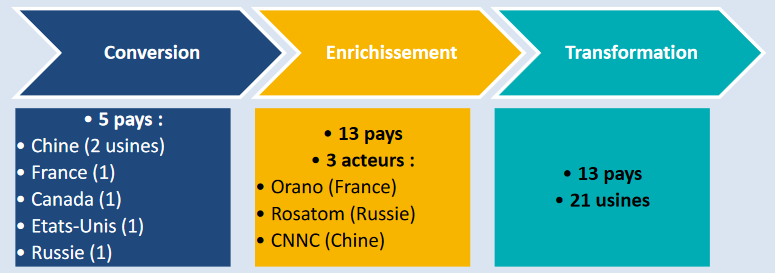
\includegraphics[width=0.8\textwidth]{Images/nucléaire/key_step_combustible.png}
    \caption{Etapes clés de la fabrication du combustible nucléaire}
    \label{fig:combustible}
\end{figure}
~\\
Le nombre de pays constructeurs de réacteurs nucléaire est assez réduit. Il pourrait augmenter avec l'avènement des Small Modular Reactor (SMR). Un pays achetant un réacteur nucléaire se place dans une relation de longue durée avec le pays constructeur. Cette relation peut devenir une relation de dépendance si le pays constructeur devient également l'opérateur du réacteur nucléaire.\smallbreak
Un contrat possible entre un pays constructeur et un pays acheteur est le contrat "Build, Own, Operate". Comme son nom l'indique, le pays constructeur devient propriétaire de la centrale, puis opérateur. Ce type de contrat est en cours entre la Russie et la Turquie pour la centrale de quatre réacteurs de Akkuyu. Pour ce contrat, la Russie finance l'intégralité de la construction puis se rembourse par la vente d'électricité (\cite{meyer_les_2021}).